\section{覆叠空间的等价}
\label{ch13-sec79}

在这一节中, 我们证明在覆叠映射某一个适当的等价概念下, 覆叠映射 $p\colon E\to B$ 完全由基本群 $\pi_{1}(B,\ b_{0})$ 的子群 $H_{0}$ 所确定.

\begin{definition}[覆叠映射的等价]
\label{definition:ch13-covering-equivalence}
设 $p\colon E\to B$ 和 $p'\colon E'\to B$ 都是覆叠映射. 若存在一个同胚 $h\colon E\to E'$ 使得 $p=p'\circ h$, 则称 $p$ 与 $p'$ 是\textbf{等价的}(equivalent). 同胚 $h$ 称为\textbf{覆叠映射之间的等价}(equivalence of covering maps), 也称为\textbf{覆叠空间之间的等价}(equivalence of covering spaces).
\end{definition}

对于两个覆叠映射 $p\colon E\to B$ 和 $p'\colon E'\to B$, 我们将证明: 如果它们的对应子群 $H_{0}$ 与 $H_{0}'$ 相同, 则存在一个等价 $h\colon E\to E'$. 为此, 我们需要推广第 54 节的提升引理.

\begin{lemma}[广义提升引理]
\label{lemma:ch13-general-lifting}
设 $p\colon E\to B$ 是一个覆叠映射, $p(e_{0})=b_{0}$. 又设 $f\colon Y\to B$ 是一个连续映射, $f(y_{0})=b_{0}$. 假定 $Y$ 是道路连通且局部道路连通的. 则 $f$ 可以被提升为映射 $\widetilde{f}\colon Y\to E$ 使得 $\widetilde{f}(y_{0})=e_{0}$ 当且仅当
\[
f_{*}(\pi_{1}(Y,y_{0}))\subset p_{*}(\pi_{1}(E,e_{0})).
\]
此外, 如果上述提升存在, 则它是唯一的.
\end{lemma}

\par
\begin{figure}[htbp]
\centering
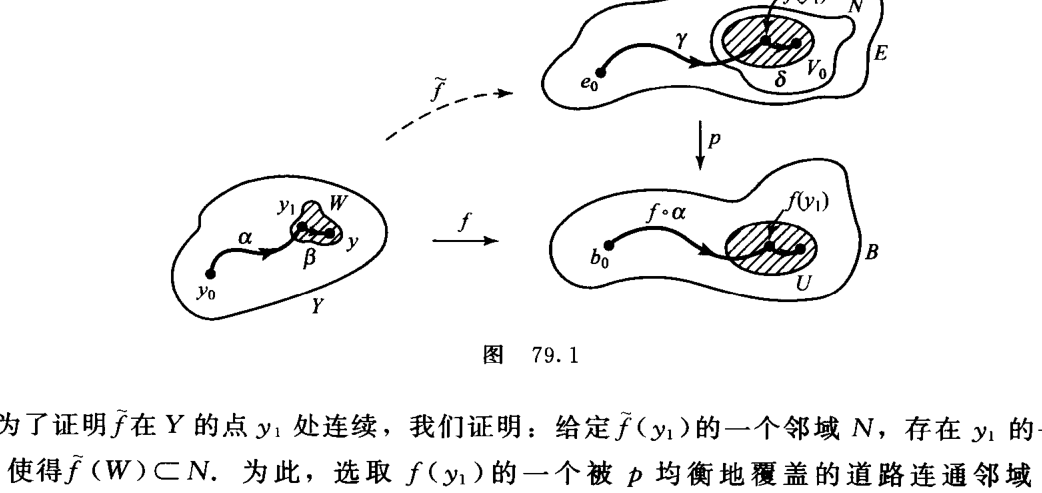
\includegraphics[width=0.8\textwidth]{image/fig-79-1.png}
\caption{广义提升引理中提升的构造.}
\label{ch13-fig-79-1}
\end{figure}

\begin{proof}
如果存在提升 $\widetilde{f}$, 则
\[
f_{*}(\pi_{1}(Y,y_{0}))=p_{*}(\widetilde{f}_{*}(\pi_{1}(Y,y_{0})))\subset p_{*}(\pi_{1}(E,e_{0})).
\]
这证明了定理的"仅当"部分.

现在我们来证明: 如果 $\widetilde{f}$ 存在, 则它是唯一的. 任意给定 $y_{1}\in Y$, 在 $Y$ 中选取一条从 $y_{0}$ 到 $y_{1}$ 的道路 $\alpha$. 考虑 $B$ 中的道路 $f\circ\alpha$, 将其提升为 $E$ 中以 $e_{0}$ 为起点的道路 $\gamma$. 如果 $f$ 的提升 $\widetilde{f}$ 存在, 则 $\widetilde{f}(y_{1})$ 必为 $\gamma$ 的终点 $\gamma(1)$, 这是由于 $\widetilde{f}\circ\alpha$ 是以 $e_{0}$ 为起点的道路 $f\circ\alpha$ 的提升, 而道路的提升是唯一的.

最后, 我们来证明定理的"当"部分. 前面的唯一性证明已经给了我们一些启示. 给定 $y_{1}\in Y$, 在 $Y$ 中选取一条从 $y_{0}$ 到 $y_{1}$ 的道路 $\alpha$. 将道路 $f\circ\alpha$ 提升为 $E$ 中一条以 $e_{0}$ 为起点的道路 $\gamma$, 并且定义 $\widetilde{f}(y_{1})=\gamma(1)$. 参见\cref{ch13-fig-79-1}. 关于 $\widetilde{f}$ 的定义确切并且与道路 $\alpha$ 的选取无关这两点留到证明的末尾讨论, 我们先在这些已经成立的假定下证明 $\widetilde{f}$ 的连续性.


为了证明 $\widetilde{f}$ 在 $Y$ 的点 $y_{1}$ 处连续, 我们证明: 给定 $\widetilde{f}(y_{1})$ 的一个邻域 $N$, 存在 $y_{1}$ 的一个邻域 $W$ 使得 $\widetilde{f}(W)\subset N$. 为此, 选取 $f(y_{1})$ 的一个被 $p$ 均衡地覆盖的道路连通邻域 $U$. 将 $p^{-1}(U)$ 分解成若干片, 并且设 $V_{0}$ 为包含 $\widetilde{f}(y_{1})$ 的那一片. 如果必要的话, 可以取 $f(y_{1})$ 的更小的邻域代替 $U$, 这样我们总可以假定 $V_{0}\subset N$. 设 $p_{0}\colon V_{0}\to U$ 为 $p$ 的限制, 则 $p_{0}$ 是一个同胚. 由于 $f$ 在 $y_{1}$ 处连续, 而 $Y$ 是局部道路连通的, 我们可以取 $y_{1}$ 的道路连通邻域 $W$ 使得 $f(W)\subset U$. 我们要证明 $\widetilde{f}(W)\subset V_{0}$, 从而完成定理的证明.

给定 $y\in W$, 在 $W$ 中选取一条从 $y_{1}$ 到 $y$ 的道路 $\beta$. 由于 $\widetilde{f}$ 的定义是确切的, $\widetilde{f}(y)$ 可以通过以下方式给出, 取从 $y_{0}$ 到 $y$ 的一条道路 $\alpha*\beta$, 将 $f\circ(\alpha*\beta)$ 提升为 $E$ 中以 $e_{0}$ 为起点的一条道路, 令 $\widetilde{f}(y)$ 为这个提升道路的终点. 现在, $\gamma$ 是 $\alpha$ 的一个提升, 它以 $e_{0}$ 为起点. 由于道路 $f\circ\beta$ 在 $U$ 中, 因此道路 $\delta=p_{0}^{-1}\circ f\circ\beta$ 是它以 $\widetilde{f}(y_{1})$ 为起点的提升. 从而 $\gamma*\delta$ 为 $f\circ(\alpha*\beta)$ 以 $e_{0}$ 为起点的提升, 其终点为 $V_{0}$ 中的点 $\delta(1)$. 因此 $\widetilde{f}(W)\subset V_{0}$.

最后, 我们证明 $\widetilde{f}$ 的定义是确切的. 设 $\alpha$ 和 $\beta$ 为 $Y$ 中连接 $y_{0}$ 和 $y_{1}$ 的两条道路. 我们必须证明: 若 $f\circ\alpha$ 和 $f\circ\beta$ 被提升为 $E$ 中两条以 $e_{0}$ 为起点的道路, 那么这两条提升的道路在 $E$ 中有相同的终点.

首先, 我们将 $f\circ\alpha$ 提升为 $E$ 中以 $e_{0}$ 起点的道路 $\gamma$, 然后将 $f\circ\bar{\beta}$ 提升为 $E$ 中以 $\gamma$ 的终点 $\gamma(1)$ 为起点的道路 $\delta$, 那么 $\gamma*\delta$ 为回路 $f\circ(\alpha*\bar{\beta})$ 的提升. 根据假设, 有
\[
f_{*}(\pi_{1}(Y,y_{0}))\subset p_{*}(\pi_{1}(E,e_{0})).
\]
因此 $[f\circ(\alpha*\bar{\beta})]$ 属于 $p_{*}$ 的像集之中. 定理 54.6 蕴涵着它的提升 $\gamma*\delta$ 是 $E$ 中的一条回路.

由此易见 $\widetilde{f}$ 的定义是确切的. 这是由于 $\bar{\delta}$ 是以 $e_{0}$ 为起点的 $f\circ\beta$ 的提升, $\gamma$ 是以 $e_{0}$ 为起点 $f\circ\alpha$ 的提升, 并且这两个提升在 $E$ 中有相同的终点.
\end{proof}

\begin{theorem}[以基点为映射的等价的存在唯一性]
\label{theorem:ch13-equivalence-same-subgroup}
设 $p\colon E\to B$ 和 $p'\colon E'\to B$ 都是覆叠映射, $p(e_{0})=p'(e_{0}')=b_{0}$, 则存在等价 $h\colon E\to E'$ 使得 $h(e_{0})=e_{0}'$ 成立当且仅当以下两个群
\[
H_{0}=p_{*}(\pi_{1}(E,e_{0}))\qquad\text{和}\qquad H_{0}'=p'_{*}(\pi_{1}(E',e_{0}'))
\]
相等. 若 $h$ 存在, 则它是唯一的.
\end{theorem}

\begin{proof}
先证明定理的"仅当"部分. 给定 $h$, $h$ 是一个同胚这一条件蕴涵着
\[
h_{*}(\pi_{1}(E,e_{0}))=\pi_{1}(E',e_{0}').
\]
由于 $p'\circ h=p$, 所以 $H_{0}=H_{0}'$.

其次证明定理的"当"部分. 假设 $H_{0}=H_{0}'$, 我们来证明 $h$ 的存在性. 我们将应用前面的引理. (四次!) 考虑映射 $p\colon E\to B$, 关于它有覆叠映射 $p'\colon E'\to B$. 因为 $p'$ 是一个覆叠映射并且 $E$ 是道路连通和局部道路连通的, 从而存在一个映射 $h\colon E\to E'$ 使得 $h(e_{0})=e_{0}'$, 并且为 $p$ 的一个提升 (即 $p'\circ h=p$). 在上述讨论中将 $E$ 和 $E'$ 的地位互换, 可见存在一个映射 $k\colon E'\to E$ 使得 $k(e_{0}')=e_{0}$ 和 $p\circ k=p'$. 考虑映射 $p\colon E\to B$ 关于它自身.

映射 $k\circ h\colon E\to E$ 是 $p$ 的一个提升 (因为 $p\circ k\circ h=p'\circ h=p$), 使得 $p(e_{0})=e_{0}$. $E$ 的恒等映射 $i_{E}$ 也是这样的一个提升. 前面的引理的唯一性意味着 $k\circ h=i_{E}$. 类似的讨论说明 $h\circ k$ 等于 $E'$ 的恒等映射.
\end{proof}

乍看起来, 关于等价性的问题似乎已经获得解决. 但是, 我们忽略了某些细节问题. 我们已得到了将 $e_{0}$ 映到 $e_{0}'$ 的等价 $h\colon E\to E'$ 存在的充分必要条件. 然而, 我们尚未确定一般来说何种条件下存在这种等价. 的确可能不存在将 $e_{0}$ 映为 $e_{0}'$ 的等价, 尽管可能有一个将 $e_{0}$ 映为 $(p')^{-1}(b_{0})$ 中另外一点 $e_{1}'$ 的等价. 是否可以通过考察子群 $H_{0}$ 和 $H_{0}'$ 来判定等价的存在性? 下面我们来考虑这个问题.

设 $H_{1}$ 和 $H_{2}$ 为群 $G$ 的子群. 让我们回顾代数学中的一些知识: 若存在某元素 $\alpha\in G$ 使得 $H_{2}=\alpha\cdot H_{1}\cdot\alpha^{-1}$, 则称 $H_{1}$ 与 $H_{2}$ \textbf{共轭}(conjugate). 换句话说, 将 $x$ 映为 $\alpha\cdot x\cdot\alpha^{-1}$ 的 $G$ 到自身的同构恰好将群 $H_{1}$ 映为群 $H_{2}$. 易见, 共轭是在 $G$ 的所有子群所构成的族上的一个等价关系. 子群 $H$ 所在的等价类称为 $H$ 的\textbf{共轭类}(conjugacy class).

\begin{lemma}[同一覆叠纤维上的子群相互共轭]
\label{lemma:ch13-conjugate-fibers}
设 $p\colon E\to B$ 是一个覆叠映射. $e_{0}$ 和 $e_{1}$ 是 $p^{-1}(b_{0})$ 中的两个点, 并且 $H_{i}=p_{*}(\pi_{1}(E,e_{i}))$.
\begin{enumerate}[(a)]
\item 若 $\gamma$ 是 $E$ 中从 $e_{0}$ 到 $e_{1}$ 的一条道路, 且 $\alpha$ 是 $B$ 中的回路 $p\circ\gamma$, 则等式 $[\alpha]*H_{1}*[\alpha]^{-1}=H_{0}$ 成立, 因此 $H_{0}$ 与 $H_{1}$ 共轭.
\item 反之, 给定 $e_{0}$ 及一个群 $\pi_{1}(B,\ b_{0})$ 中与 $H_{0}$ 共轭的子群 $H$, 则存在 $p^{-1}(b_{0})$ 的一个点 $e_{1}$ 使得 $H_{1}=H$.
\end{enumerate}
\end{lemma}

\par
\begin{figure}[htbp]
\centering
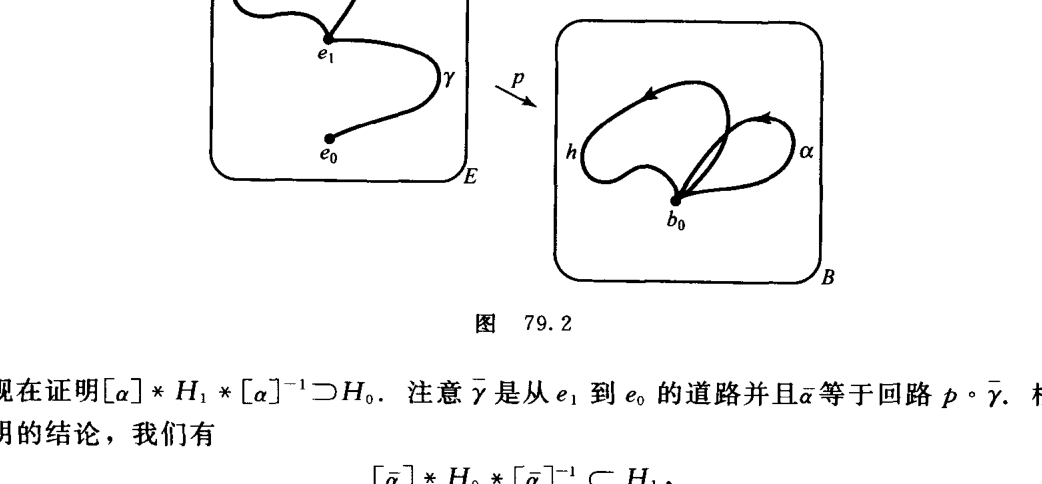
\includegraphics[width=0.8\textwidth]{image/fig-79-2.png}
\caption{同一覆叠纤维上两个点对应子群的共轭性.}
\label{ch13-fig-79-2}
\end{figure}

\begin{proof}
(a) 首先证明 $[\alpha]*H_{1}*[\alpha]^{-1}\subset H_{0}$. 给定 $[h]$ 为 $H_{1}$ 中的一个元素, 则对于 $E$ 中以 $e_{1}$ 为基点的某一条回路 $\widetilde{h}$ 有 $[h]=p_{*}([\widetilde{h}])$. 设 $\widetilde{k}$ 表示道路 $\widetilde{k}=(\gamma*\widetilde{h})*\bar{\gamma}$, 则 $\widetilde{k}$ 是 $E$ 中以 $e_{0}$ 为基点的一条回路, 并且
\[
p_{*}([\widetilde{k}])=[(\alpha*h)*\bar{\alpha}]=[\alpha]*[h]*[\alpha]^{-1},
\]
从而等式右边的元素属于 $p_{*}(\pi_{1}(E,e_{0}))=H_{0}$, 这便是我们所要证明的. 参见\cref{ch13-fig-79-2}.


现在证明 $[\alpha]*H_{1}*[\alpha]^{-1}\supset H_{0}$. 注意 $\bar{\gamma}$ 是从 $e_{1}$ 到 $e_{0}$ 的道路并且 $\bar{\alpha}$ 等于回路 $p\circ\bar{\gamma}$. 根据上面证明的结论, 我们有
\[
[\bar{\alpha}]*H_{0}*[\bar{\alpha}]^{-1}\subset H_{1},
\]
这便是我们所要证明的.

(b) 为得到相反的蕴涵关系, 给定 $e_{0}$ 并设 $H$ 共轭于 $H_{0}$, 则对以 $b_{0}$ 为基点的 $B$ 中的某一条回路 $\alpha$ 有 $H_{0}=[\alpha]*H*[\alpha]^{-1}$. 设 $E$ 中以 $e_{0}$ 为起点的道路 $\gamma$ 是 $\alpha$ 的提升, 并且设 $e_{1}=\gamma(1)$, 则 (a) 蕴涵着 $H_{0}=[\alpha]*H_{1}*[\alpha]^{-1}$. 因此 $H=H_{1}$.
\end{proof}

\begin{theorem}[覆叠空间等价的共轭类判别]
\label{theorem:ch13-equivalence-conjugacy}
设 $p\colon E\to B$ 和 $p'\colon E'\to B$ 是两个覆叠映射, $p(e_{0})=p'(e_{0}')=b_{0}$. 覆叠映射 $p$ 和 $p'$ 等价当且仅当 $\pi_{1}(B,\ b_{0})$ 的子群
\[
H_{0}=p_{*}(\pi_{1}(E,e_{0}))\qquad\text{与}\qquad H_{0}'=p'_{*}(\pi_{1}(E',e_{0}'))
\]
共轭.
\end{theorem}

\begin{proof}
设 $h\colon E\to E'$ 是一个等价, $e_{1}'=h(e_{0})$, 并且令 $H_{1}'=p_{*}(\pi_{1}(E',\ e_{1}'))$. 由 \cref{theorem:ch13-equivalence-same-subgroup} 可见 $H_{0}=H_{1}'$. 前一个引理告诉我们 $H_{1}'$ 共轭于 $H_{0}'$.

反之, 若群 $H_{0}$ 共轭于 $H_{0}'$, 前一个引理蕴涵着: 存在 $E'$ 的一个点 $e'$ 使得 $H_{1}'=H_{0}$. 根据 \cref{theorem:ch13-equivalence-same-subgroup}, 存在一个等价 $h\colon E\to E'$ 使得 $h(e_{0})=e_{1}'$.
\end{proof}

\begin{example}[圆周的覆叠空间]
\label{example:ch13-circle-coverings}
考虑圆周 $B=S^{1}$ 的覆叠空间. 因为 $\pi_{1}(B,\ b_{0})$ 是阿贝尔群, $\pi_{1}(B,\ b_{0})$ 中的两个子群共轭当且仅当它们相等. 因此, $B$ 的两个覆叠映射等价当且仅当它们对应着 $\pi_{1}(B,\ b_{0})$ 的同一个子群.

我们知道 $\pi_{1}(B,\ b_{0})$ 同构于整数加群 $\mathbb{Z}$. $\mathbb{Z}$ 有哪些子群? 近世代数中的一个标准的结论告诉我们: $\mathbb{Z}$ 的非平凡的子群 $G_{n}$ 必定是由某一正整数 $n\in\mathbb{Z}_{+}$ 的所有倍数所组成的.

我们已经研究过圆周的一个覆叠空间, 其覆叠映射为 $p\colon\mathbb{R}\to S^{1}$. 由于 $\mathbb{R}$ 是单连通的, 因此这个空间只能对应 $\pi_{1}(S^{1},\ b_{0})$ 的平凡子群. 我们也曾经考虑过覆叠映射 $p\colon S^{1}\to S^{1}$, 定义为 $p(z)=z^{n}$, 其中 $z$ 为复数. 对于这种情形, 映射 $p_{*}$ 将 $\pi_{1}(S^{1},\ b_{0})$ 的一个生成元映为自身的 $n$ 次. 因此, 参照 $\pi_{1}(S^{1},\ b_{0})$ 到 $\mathbb{Z}$ 的标准同构, 群 $p_{*}(\pi_{1}(S^{1},\ b_{0}))$ 对应的是 $\mathbb{Z}$ 的子群 $G_{n}$.

根据上述定理可见: $S^{1}$ 的每一个道路连通的覆叠空间与上述某一覆叠空间等价.
\end{example}

\begin{exercise}
\label{exercise:ch13-sec79-01}
证明: 当 $n>1$ 时, 每一个连续映射 $f\colon S^{n}\to S^{1}$ 都是零伦的. [提示: 应用提升引理.]
\end{exercise}

\begin{exercise}
\label{exercise:ch13-sec79-02}
\begin{enumerate}[(a)]
\item 证明每一个连续映射 $f\colon P^{2}\to S^{1}$ 都是零伦的.
\item 给出从环面到 $S^{1}$ 中的一个不是零伦的连续映射.
\end{enumerate}
\end{exercise}

\begin{exercise}
\label{exercise:ch13-sec79-03}
设 $p\colon E\to B$ 是一个覆叠映射, $p(e_{0})=b_{0}$. 证明 $H_{0}=p_{*}(\pi_{1}(E,\ e_{0}))$ 是 $\pi_{1}(B,\ b_{0})$ 的正规子群当且仅当对于 $p^{-1}(b_{0})$ 中的每一对点 $e_{1}$, $e_{2}$, 有一个等价 $h\colon E\to E$ 使得 $h(e_{1})=e_{2}$.
\end{exercise}

\begin{exercise}
\label{exercise:ch13-sec79-04}
设 $T=S^{1}\times S^{1}$ 为环面. 有一个由投射诱导的 $\pi_{1}(T,\ b_{0}\times b_{0})$ 到 $\mathbb{Z}\times\mathbb{Z}$ 的两个因子上的同构.
\begin{enumerate}[(a)]
\item 找出 $T$ 的一个覆叠空间, 要求这个覆叠空间对应着 $\mathbb{Z}\times\mathbb{Z}$ 中由元素 $m\times 0$ 所生成的子群, 其中 $m$ 为正整数.
\item 找出 $T$ 的一个覆叠空间, 要求这个覆叠空间对应着 $\mathbb{Z}\times\mathbb{Z}$ 中的平凡子群.
\item 找出 $T$ 的一个覆叠空间, 要求这个覆叠空间对应着 $\mathbb{Z}\times\mathbb{Z}$ 中由 $m\times 0$ 和 $0\times n$ 所生成的子群, 其中 $m$ 和 $n$ 都是正整数.
\end{enumerate}
\end{exercise}

\begin{exercise}
\label{exercise:ch13-sec79-05}
设 $T=S^{1}\times S^{1}$ 为环面, $x_{0}=b_{0}\times b_{0}$.
\begin{enumerate}[(a)]
\item 证明以下定理:
\end{enumerate}

\begin{theorem}[环面的自同构]
\label{theorem:ch13-torus-automorphism}
每一个 $\pi_{1}(T,\ x_{0})$ 到自身的同构都是由将 $x_{0}$ 映为 $x_{0}$ 的从 $T$ 到自身的同胚诱导出来的.
\end{theorem}
\end{exercise}

\begin{exercise}
\label{exercise:ch13-sec79-05b}
\textbf{(b)} 证明以下定理.

\begin{theorem}[环面覆叠空间的分类]
\label{theorem:ch13-torus-covering-classification}
若 $E$ 是 $T$ 的一个覆叠空间, 则 $E$ 或者同胚于 $\mathbb{R}^{2}$, 或者同胚于 $S^{1}\times\mathbb{R}$, 或者同胚于 $T$.
\end{theorem}
[提示: 可以应用代数学中的以下结论: 若 $F$ 是秩为 $2$ 的自由阿贝尔群, $N$ 是一个非平凡的子群, 则 $F$ 有一个基 $a_{1}$, $a_{2}$ 使得或者 (1) 对于某正整数 $m$, $ma_{1}$ 为 $N$ 的一个基, 或者 (2) $ma_{1}$, $na_{2}$ 是 $N$ 的一个基, 其中 $m$ 和 $n$ 都是正整数.]
\end{exercise}

\begin{exercise}
\label{exercise:ch13-sec79-06}
证明以下定理.

\begin{theorem}[拓扑群的覆叠空间诱导群结构]
\label{theorem:ch13-covering-topological-group}
设 $G$ 是一个拓扑群, 其乘法运算为 $m\colon G\times G\to G$, 单位元为 $e$. 假设 $p\colon\widetilde{G}\to G$ 是一个覆叠映射. 给定 $\widetilde{e}$ 使得 $p(\widetilde{e})=e$, 则在 $\widetilde{G}$ 中有唯一的一个乘法运算使它成为一个拓扑群, 使得 $\widetilde{e}$ 是这个拓扑群中的单位元, 并且 $p$ 是一个同态.
\end{theorem}
证明: 根据我们的约定, 这里 $G$ 和 $\widetilde{G}$ 都是道路连通和局部道路连通的.
\begin{enumerate}[(a)]
\item 设 $I\colon G\to G$ 为映射, 其定义为 $I(g)=g^{-1}$. 证明存在唯一的映射 $\widetilde{m}\colon\widetilde{G}\times\widetilde{G}\to\widetilde{G}$ 和唯一的映射 $\widetilde{I}\colon\widetilde{G}\to\widetilde{G}$, $\widetilde{m}(\widetilde{e}\times\widetilde{e})=\widetilde{e}$, $\widetilde{I}(\widetilde{e})=\widetilde{e}$, 使得 $p\circ\widetilde{m}=\widetilde{m}\circ(p\times p)$ 以及 $p\circ\widetilde{I}=I\circ p$ 成立.
\item 证明定义为 $\widetilde{g}\mapsto\widetilde{m}(\widetilde{e}\times\widetilde{g})$ 和 $\widetilde{g}\mapsto\widetilde{m}(\widetilde{g}\times\widetilde{e})$ 的两个映射 $\widetilde{G}\to\widetilde{G}$ 都等于 $\widetilde{G}$ 的恒等映射. [提示: 应用 \cref{lemma:ch13-general-lifting} 中的唯一性.]
\item 证明由 $\widetilde{g}\mapsto\widetilde{m}(\widetilde{g}\times\widetilde{I}(\widetilde{g}))$ 和 $\widetilde{g}\mapsto\widetilde{m}(\widetilde{I}(\widetilde{g})\times\widetilde{g})$ 定义的两个映射 $\widetilde{G}\to\widetilde{G}$ 都把 $\widetilde{G}$ 映为 $\widetilde{e}$.
\item 分别由
\[
\widetilde{g}\times\widetilde{g}'\times\widetilde{g}''\to\widetilde{m}(\widetilde{g}\times\widetilde{m}(\widetilde{g}'\times\widetilde{g}''))
\]
和
\[
\widetilde{g}\times\widetilde{g}'\times\widetilde{g}''\to\widetilde{m}(\widetilde{m}(\widetilde{g}\times\widetilde{g}')\times\widetilde{g}'')
\]
定义的两个映射 $\widetilde{G}\times\widetilde{G}\times\widetilde{G}\to\widetilde{G}$ 是相等的.
\item 完成定理的证明.
\end{enumerate}
\end{exercise}

\begin{exercise}
\label{exercise:ch13-sec79-07}
设覆叠映射 $p\colon\widetilde{G}\to G$ 是拓扑群之间的一个同态. 证明: 若 $G$ 是阿贝尔群, 则 $\widetilde{G}$ 也是阿贝尔群.
\end{exercise}
